\documentclass[11pt]{article}
\usepackage[top=1.00in, bottom=1.0in, left=1in, right=1in]{geometry}
\renewcommand{\baselinestretch}{1.1}
\usepackage{graphicx}
\usepackage{natbib}
\usepackage{amsmath}
\usepackage{hyperref}
\usepackage{parskip}

\def\labelitemi{--}
\parindent=0pt

\begin{document}
\renewcommand{\refname}{\CHead{}}

% \setlength{\parindent}{0cm}
% \setlength{\parskip}{5pt}

\title{How climate change breaks a fundamental model of plant biology to degrade plant forecasting} 
\author{Jonathan Auerbach, E.M. Wolkovich plus others possible} % also possibly: Victor van der Meersch
\date{\today}
\maketitle

\section{Outline}

\begin{enumerate}
\item Introduction
\begin{enumerate}
\item Climate change is shifting biological systems globally with potential impacts on ecosystem stability and the global climate system itself \citep{richardson2023earth}
\begin{enumerate}
\item The most observed and well documented biological impact is shifts in phenology----the timing of recurring life history events \citep{ipcc2022,Menzel1999,Root:2003kl}
\item Shifted phenology has been the clearest `fingerprint' of anthropogenic climate change, it may also be the one to first show evidence that systems are no longer responding to climate change as they did in the past \citep{piao2019plant,vitasse2022great}
\item Such a phase change or tipping point \citep{Dakos2013} have been seen in other human-altered systems (but understanding why they happen and predicting them has been difficult) \citep{Chavez2003}
\item Understanding and predicting this has big consequences for global carbon models (will plants sequester more carbon?), economic models of crops (peach frost etc.) and more... \citep{chamberlain2021climate,zohner2020late,lamichhane2021rising}
\end{enumerate}
\item Research is divided on whether phenological responses are showing hints of new responses \citep{fu2015declining,gusewell2017changes} or not \citep{wolkovich2021simple}, which may because we lack an underlying model
\begin{enumerate}
\item Declining sensitivities, or not
\item Increasing variance, or not
\item Related to this, are trees growing more with longer seasons, or not (or maybe we just focus on phenology) \citep{dow2022warm,keenan2014net}
\item These debates stem from lacking an underlying model that we all agree on (and we don't have great data)
\end{enumerate}
\item Here we show how shifted autocorrelation in climate (or do we want to call it `biological climate' or something to represent that it's the GDD metric? Though I am not a fan of new names/terms) due to anthropogenic climate change predicts a breakdown of one of the most fundamental models of plant biology and show how it may lead to a decline in forecasting accuracy .... 
\item We show results with lilacs
\item And with other data
\item Our results suggest climate change has fundamentally disrupted the central limit theory for one of the most important biological models with consequences for higher variance and lower predictability from crops to forests and likely extends to upper trophic levels as well. 
\end{enumerate}
\item Results \& Discussion
\begin{enumerate}
\item We found ...
\item Changes in autocorrelation in climate already observed (maybe muse on shifts in min versus max, vs mean)
\end{enumerate}
\item Methods
\begin{enumerate}
\item Longer form of the model
\item Methods for lilac data
\item Methods for other datasets (PEP725, Oak in UK, cherry blossoms)
\end{enumerate}
\end{enumerate}
\end{enumerate}

Stuff I think we should try to fit in somewhere ... 
\begin{enumerate}
\item Ecologists are really into increased environmental variation (since it does cool stuff in our deterministic models of the world), but we show that decreasing environmental variation -- increases in autocorrelation -- could actually be what is happening (and it's more interesting) \citet{drake2005population,lawson2015environmental,vasseur2014increased}
\end{enumerate}


Some thoughts of stuff that could be related to shifting variance as we suggest here ... 
\begin{enumerate}
\item More wide-spread frost events (because plants all budburst over larger spatial areas at the same time) 
\end{enumerate}

Stuff worth checking out: 
\begin{itemize}
\item Paper on variance and phenology ... \href{https://esajournals.onlinelibrary.wiley.com/doi/full/10.1002/ecy.3846}{Disorder or a new order: How climate change affects phenological variability}
\item Autocorrelation (on a different temporal scale I assume) used to help identify human-cased climate change \href{https://www.science.org/doi/full/10.1126/science.282.5394.1676}{Anthropogenic Influence on the Autocorrelation Structure of Hemispheric-Mean Temperatures} and \href{https://www.science.org/doi/full/10.1126/science.1999.285.5427.495a}{replies}.
\item \href{https://www.nature.com/articles/s41598-018-33217-0}{Increased spatial and temporal autocorrelation of temperature under climate change}
\begin{enumerate}
\item 
\end{enumerate}


\bibliographystyle{unsrt}
\bibliography{..//refs/wrongdoomsday}

\clearpage
\section{Figures}

\begin{figure}[h!]
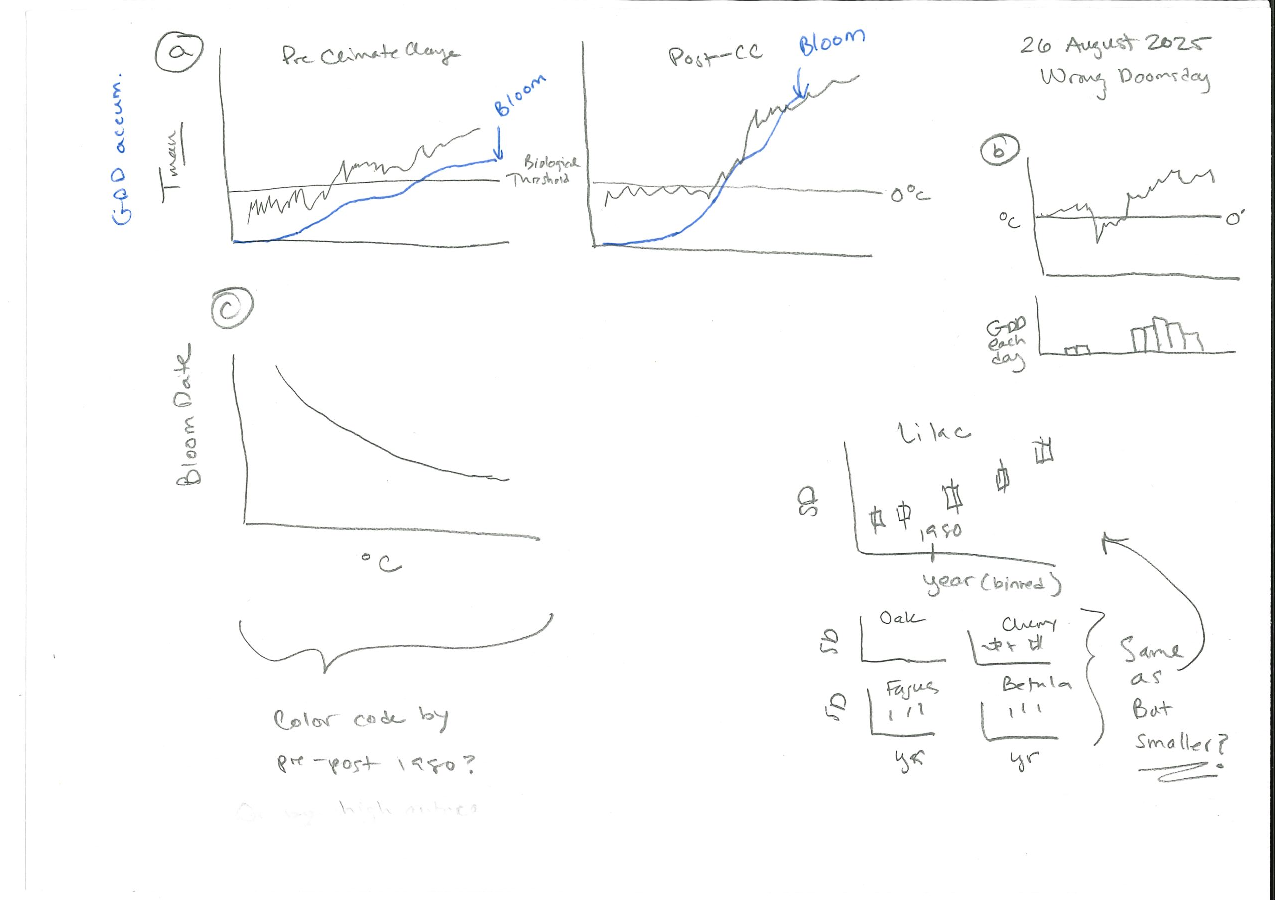
\includegraphics[width=0.95\textwidth]{figures/figideasAug2025.pdf}
\caption{Ideas for figures: I started with a) as a conceptual figure to explain the problem but it's not great, we may need something like b) which would show climate, then daily GDD units and then the sum somehow. Some version of c) seems useful I think? I think we'll have to somehow show the trends in leafout over time and then I forgot to label the lower right bit that would be the main results. I am just riffing (and open to all ideas, obviously). } 
\label{fig:figname}
\end{figure}

\end{document}

